% MH1812 — Chapter 1: Logic (0->100 ground-up)
\chapter[Logic]{Logic: Propositions, Truth Tables, Predicates and Quantifiers}
\label{ch:logic}

\begin{quote}
\emph{``Logic is the anatomy of thought.''} --- John Locke. Every program branch, loop condition, and database query is a logical formula. We build logic from everyday language to formal syntax.
\end{quote}

\noindent\fbox{\parbox{\dimexpr\linewidth-2\fboxsep-2\fboxrule}{%
\textbf{From zero: no prior logic assumed.} We start with ordinary sentences (``It is raining''), turn them into symbols, build truth tables as exhaustive checklists, then lift to predicates with variables and quantifiers. Pictures precede formalism.}}
\vspace{0.4em}

\section*{Learning Outcomes}
After this chapter you will be able to:
\begin{enumerate}[label=(L\arabic*)]
    \item distinguish propositions from non-propositions and translate English to propositional formulae;
    \item build and use truth tables to test tautology, contradiction, and logical equivalence;
    \item apply De Morgan, distributive, and implication equivalences in proofs and simplifications;
    \item formalise statements with predicates and quantifiers $\forall,\exists$;
    \item negate quantified statements correctly and explain quantifier-order dependence.
\end{enumerate}

% ============================================================
\section{Propositions and Connectives}
\label{sec:propositions}
A \emph{proposition} is a declarative sentence that is either true (T) or false (F) --- no maybe, no command, no question. ``$2+2=4$'' is T; ``$2+2=5$'' is F; ``Are you there?'' is not a proposition; ``$x+1=3$'' is not until $x$ is bound.

We combine propositions with \emph{connectives}. Intuition: think of switches.
\begin{center}
\begin{tabular}{ccl}
\toprule
Symbol & Name & Intuition \\ \midrule
$\neg p$ & not $p$ & flip the switch \\
$p\land q$ & $p$ and $q$ & both lights on \\
$p\lor q$ & $p$ or $q$ & at least one on (inclusive) \\
$p\to q$ & if $p$ then $q$ & promise: $p$ true forces $q$ true \\
$p\leftrightarrow q$ & $p$ iff $q$ & same truth value \\ \bottomrule
\end{tabular}
\end{center}

\begin{figure}[h]\centering
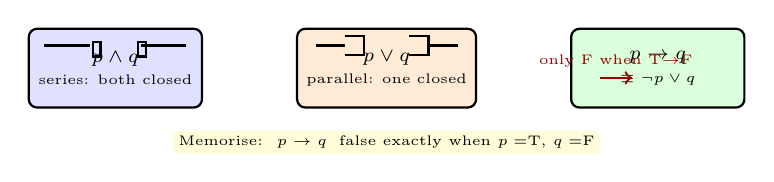
\begin{tikzpicture}[scale=0.82,every node/.style={font=\scriptsize}]
% Switch analogy for AND/OR
\node[draw,thick,rounded corners=3pt,fill=blue!12,minimum width=2.2cm,minimum height=1.0cm,align=center] (and) at (0,0) {$p \land q$\\{\tiny series: both closed}};
\draw[thick] (-1.1,0.35)--(-0.4,0.35); \draw[thick] (0.4,0.35)--(1.1,0.35);
\foreach \x in {-0.35,0.35} {\draw[thick] (\x,0.18) rectangle++(0.12,0.22);}
\node[draw,thick,rounded corners=3pt,fill=orange!16,minimum width=2.2cm,minimum height=1.0cm,align=center] (or) at (4.2,0) {$p \lor q$\\{\tiny parallel: one closed}};
\draw[thick] (3.1,0.35)--(3.55,0.35); \draw[thick] (4.85,0.35)--(5.3,0.35);
\draw[thick] (3.55,0.5)--(3.85,0.5)--(3.85,0.2)--(3.55,0.2);
\draw[thick] (4.55,0.5)--(4.85,0.5)--(4.85,0.2)--(4.55,0.2);
\node[draw,thick,rounded corners=3pt,fill=green!14,minimum width=2.2cm,minimum height=1.0cm,align=center] (imp) at (8.4,0) {$p\to q$\\{\tiny $\equiv\neg p\lor q$}};
\draw[thick,->,red!60!black] (7.5,-0.15)--(8.0,-0.15) node[midway,above,font=\tiny] {only F when T$\to$F};
\node[font=\tiny,fill=yellow!15,rounded corners=2pt,inner sep=2pt] at (4.2,-1.15) {Memorise: $\;p\to q\;$ false exactly when $p=$T, $q=$F};
\end{tikzpicture}
\caption{Intuition for connectives: series (AND), parallel (OR), and the promise reading of implication.}
\label{fig:connectives}
\end{figure}

\begin{definition}[Well-formed formula]
Atomic propositions $p,q,r,\dots$ are formulae; if $F,G$ are formulae so are $\neg F$, $(F\land G)$, $(F\lor G)$, $(F\to G)$, $(F\leftrightarrow G)$.
\end{definition}

\section{Truth Tables as Exhaustive Checklists}
\label{sec:truth-tables}
A truth table lists every assignment to the variables ($2^n$ rows for $n$ variables) and computes stepwise. This is brute-force semantics --- slow but absolute.

\begin{figure}[h]\centering
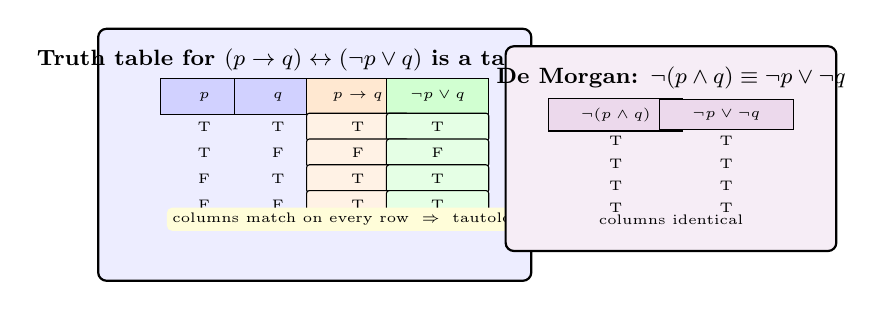
\begin{tikzpicture}[scale=0.78,every node/.style={font=\scriptsize}]
% Truth table visualization with colors
\node[draw,thick,fill=blue!7,rounded corners=3pt,minimum width=5.5cm,minimum height=3.2cm] (box) at (0,0) {};
\node[font=\footnotesize\bfseries] at (0,1.55) {Truth table for $(p\to q)\leftrightarrow(\neg p\lor q)$ is a tautology};
% header
\node[font=\tiny\bfseries,fill=blue!18,draw,minimum width=1.1cm,minimum height=0.45cm] at (-1.8,0.95) {$p$};
\node[font=\tiny\bfseries,fill=blue!18,draw,minimum width=1.1cm,minimum height=0.45cm] at (-0.6,0.95) {$q$};
\node[font=\tiny\bfseries,fill=orange!18,draw,minimum width=1.3cm,minimum height=0.45cm] at (0.7,0.95) {$p\to q$};
\node[font=\tiny\bfseries,fill=green!18,draw,minimum width=1.3cm,minimum height=0.45cm] at (2.0,0.95) {$\neg p\lor q$};
% rows
\foreach \i/\pv/\qv/\av/\bv in {0/T/T/T/T,1/T/F/F/F,2/F/T/T/T,3/F/F/T/T} {
  \pgfmathsetmacro{\y}{0.45 - \i*0.42}
  \node[font=\tiny,minimum width=1.1cm] at (-1.8,\y) {\pv};
  \node[font=\tiny,minimum width=1.1cm] at (-0.6,\y) {\qv};
  \node[font=\tiny,minimum width=1.3cm,fill=orange!10,draw,rounded corners=1pt] at (0.7,\y) {\av};
  \node[font=\tiny,minimum width=1.3cm,fill=green!10,draw,rounded corners=1pt] at (2.0,\y) {\bv};
}
\node[font=\tiny,fill=yellow!15,rounded corners=2pt,inner sep=2pt] at (0.6,-1.05) {columns match on every row $\;\Rightarrow\;$ tautology};
% check marks
\foreach \i in {0,...,3} {\pgfmathsetmacro{\y}{0.45 - \i*0.42} \node[font=\tiny,green!60!black] at (2.95,\y) {\checkmark};}
% second small table on right for De Morgan
\begin{scope}[xshift=5.8cm]
\node[draw,thick,fill=violet!7,rounded corners=3pt,minimum width=4.2cm,minimum height=2.6cm] at (0,0.1) {};
\node[font=\footnotesize\bfseries] at (0,1.25) {De Morgan: $\neg(p\land q)\equiv\neg p\lor\neg q$};
\foreach \i/\a in {0/$\neg(p\land q)$,1/$\neg p\lor\neg q$} {
  \node[font=\tiny,fill=violet!15,draw,minimum width=1.7cm,minimum height=0.38cm] at (\i*1.8-0.9,0.65) {\a};
}
\foreach \i in {0,...,3} {\pgfmathsetmacro{\y}{0.22 - \i*0.36} \node[font=\tiny] at (-0.9,\y) {T}; \node[font=\tiny] at (0.9,\y) {T};}
\node[font=\tiny] at (0,-1.05) {columns identical};
\end{scope}
\end{tikzpicture}
\caption{Truth tables: structure and the two canonical equivalences every CS student must know.}
\label{fig:truth-table}
\end{figure}

\begin{definition}[Tautology, contradiction, contingency]
A formula true on every row is a \emph{tautology} ($\top$); false on every row a \emph{contradiction} ($\bot$); otherwise \emph{contingent}.
\end{definition}

Key equivalences (verify by table):
\begin{align*}
p\to q &\equiv \neg p\lor q \equiv \neg q\to\neg p &&\text{(implication / contrapositive)}\\
\neg(p\land q) &\equiv \neg p\lor\neg q,\quad \neg(p\lor q)\equiv\neg p\land\neg q &&\text{(De Morgan)}\\
p\land(q\lor r) &\equiv(p\land q)\lor(p\land r) &&\text{(distributivity)}\\
p\leftrightarrow q &\equiv(p\to q)\land(q\to p). &&
\end{align*}

\begin{example}[Implication is not causation]
``If it rains then the road is wet'' ($r\to w$) is false only when it rains and the road stays dry. Wet road without rain does not falsify it. This matches $\neg r\lor w$.
\end{example}

% ============================================================
\section{Predicates and Quantifiers}
\label{sec:predicates}
A \emph{predicate} $P(x)$ is a sentence with a variable: truth depends on $x$. Domain $D$ matters. $P(x):$ ``$x>3$'' over $D=\mathbb{N}$ is T for $5$, F for $2$.

\begin{figure}[h]\centering
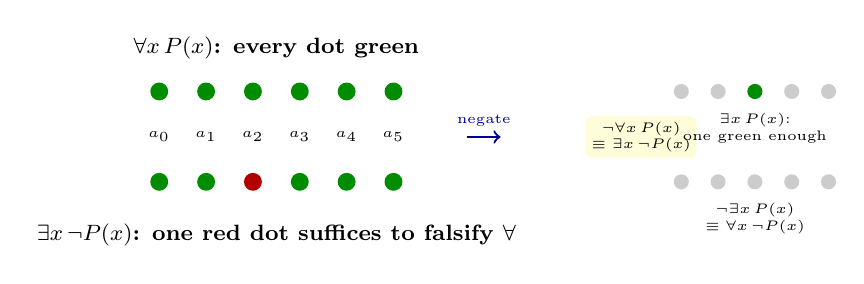
\begin{tikzpicture}[scale=0.85,every node/.style={font=\scriptsize}]
% Domain dots coloring for forall/exists
\foreach \i in {0,...,5} {\fill[green!55!black] (\i*0.7,0.8) circle (3.8pt); \node[font=\tiny,below] at (\i*0.7,0.35) {$a_{\i}$};}
\node[font=\footnotesize\bfseries] at (1.75,1.45) {$\forall x\,P(x)$: every dot green};
\foreach \i in {0,...,5} {\pgfmathsetmacro{\col}{\i==2 ? "red!70!black" : "green!55!black"} \fill[\col] (\i*0.7,-0.55) circle (3.8pt);}
\node[font=\footnotesize\bfseries] at (1.75,-1.35) {$\exists x\,\neg P(x)$: one red dot suffices to falsify $\forall$};
\draw[->,thick,blue!60!black] (4.6,0.12)--(5.1,0.12) node[midway,above,font=\tiny] {negate};
\node[font=\tiny,align=center,fill=yellow!15,rounded corners=2pt,inner sep=2pt] at (7.2,0.12) {$\neg\forall x\,P(x)$\\$\equiv\exists x\,\neg P(x)$};
% second row: exists vs for all negation
\begin{scope}[xshift=7.8cm,yshift=0.8cm]
\foreach \i in {0,...,4} {\fill[gray!40] (\i*0.55,0) circle (3.2pt);}
\fill[green!55!black] (2*0.55,0) circle (3.2pt);
\node[font=\tiny,align=center] at (1.1,-0.55) {$\exists x\,P(x)$:\\one green enough};
\end{scope}
\begin{scope}[xshift=7.8cm,yshift=-0.55cm]
\foreach \i in {0,...,4} {\fill[gray!40] (\i*0.55,0) circle (3.2pt);}
\node[font=\tiny,align=center] at (1.1,-0.55) {$\neg\exists x\,P(x)$\\$\equiv\forall x\,\neg P(x)$};
\end{scope}
\end{tikzpicture}
\caption{Quantifiers as dot-colouring. Negation swaps $\forall\leftrightarrow\exists$ and flips the predicate --- the most common bug.}
\label{fig:quantifiers}
\end{figure}

\begin{definition}[Quantifiers]
$\forall x\in D,\,P(x)$ means $P(x)$ holds for every $x\in D$. $\exists x\in D,\,P(x)$ means for at least one $x\in D$. Quantified formulae are propositions.
\end{definition}

Negation swaps quantifiers:
\[
\neg\forall x\,P(x)\equiv\exists x\,\neg P(x),\qquad
\neg\exists x\,P(x)\equiv\forall x\,\neg P(x).
\]
Iterate for blocks: $\neg\forall x\exists y\,P(x,y)\equiv\exists x\forall y\,\neg P(x,y)$.

\begin{example}[Order matters]
Over $\mathbb{R}$, $\forall x\exists y\,(x+y=0)$ is true (take $y=-x$), but $\exists y\forall x\,(x+y=0)$ is false (no single $y$ works for all $x$). Swapping quantifiers is not free.
\end{example}

Nested quantifiers model real CS specs: ``Every input has some output such that \dots'' is $\forall\text{input}\,\exists\text{output}\,P$.


\begin{lstlisting}[language=Python]
# Checking tautology by brute force (2^n rows) -- mirrors truth tables
import itertools
def is_tautology(n, f):
    for vals in itertools.product([False, True], repeat=n):
        if not f(*vals):
            return False, vals
    return True, None

# Example: (p -> q) <-> (~p or q) is a tautology
print(is_tautology(2, lambda p,q: ( (not p or q) == (not p or q) )))
\end{lstlisting}

\begin{remark}[Translating English]
``Every student who owns a laptop passed'' $=\forall s\,(\text{Owns}(s)\to\text{Passed}(s))$, not $\forall s\,(\text{Owns}(s)\land\text{Passed}(s))$. The $\to$ restricts the claim to laptop-owners.
\end{remark}


\begin{example}[De Morgan in code]
In Python/Java, \texttt{!(a \&\& b)} should be rewritten as \texttt{!a || !b}. Many bug fixes are just De Morgan. Truth tables guarantee correctness of such rewrites.
\end{example}

\begin{lemma}[Contrapositive equivalence]
$p\to q\equiv\neg q\to\neg p$. Proof by table or via $\neg p\lor q$: $\neg q\to\neg p\equiv\neg(\neg q)\lor\neg p\equiv q\lor\neg p\equiv\neg p\lor q$.
\end{lemma}

\subsection{Normal Forms}
Every formula has a \emph{conjunctive normal form} (CNF): an AND of OR-clauses, e.g.\ $(p\lor\neg q)\land(r\lor q)$. CNF underlies SAT solvers that power hardware verification. Dually, \emph{disjunctive normal form} (DNF) is an OR of AND-terms. Conversion uses distributive and De Morgan laws repeatedly.


\begin{example}[Tautology via equivalences]
$(p\to q)\land(q\to r)\to(p\to r)$ is a tautology (hypothetical syllogism). Proof: chain $\neg p\lor q$, $\neg q\lor r$ resolves to $\neg p\lor r$.
\end{example}

\begin{remark}[Biconditional as two directions]
$p\leftrightarrow q$ is often proved by two subproofs $p\to q$ and $q\to p$. In code this is \texttt{assert (p==q)} checked both ways.
\end{remark}

\begin{theorem}[Exportation]
$(p\land q)\to r\equiv p\to(q\to r)$. Currying in functional programming is this equivalence.
\end{theorem}

Intuition: a proposition is like a light switch, either on or off, never in-between.
In code, an if-condition is precisely a proposition evaluated at run time.
Truth tables are exhaustive: with $n$ variables we must check all $2^n$ assignments.
Equivalence $p\to q\equiv\neg p\lor q$ explains why \texttt{if (p) q} can be rewritten as \texttt{if (!p || q)}.
De Morgan is the formal justification for pushing negations inside brackets.
Quantifiers turn predicates with holes into full propositions by binding the holes.
The order $\forall x\exists y$ versus $\exists y\forall x$ is as different as every person has a mother versus there is a mother of everyone.
Translating word problems to symbols is half the battle in discrete mathematics.
A common error is to write $\forall x(P(x)\land Q(x))$ when $\forall x(P(x)\to Q(x))$ was intended.
Practice negating statements aloud to internalise the swap-and-flip rule.
Intuition: a proposition is like a light switch, either on or off, never in-between.
In code, an if-condition is precisely a proposition evaluated at run time.
Truth tables are exhaustive: with $n$ variables we must check all $2^n$ assignments.
Equivalence $p\to q\equiv\neg p\lor q$ explains why \texttt{if (p) q} can be rewritten as \texttt{if (!p || q)}.
De Morgan is the formal justification for pushing negations inside brackets.
Quantifiers turn predicates with holes into full propositions by binding the holes.
The order $\forall x\exists y$ versus $\exists y\forall x$ is as different as every person has a mother versus there is a mother of everyone.
Translating word problems to symbols is half the battle in discrete mathematics.
A common error is to write $\forall x(P(x)\land Q(x))$ when $\forall x(P(x)\to Q(x))$ was intended.
Practice negating statements aloud to internalise the swap-and-flip rule.
Intuition: a proposition is like a light switch, either on or off, never in-between.
In code, an if-condition is precisely a proposition evaluated at run time.
Truth tables are exhaustive: with $n$ variables we must check all $2^n$ assignments.
Equivalence $p\to q\equiv\neg p\lor q$ explains why \texttt{if (p) q} can be rewritten as \texttt{if (!p || q)}.
De Morgan is the formal justification for pushing negations inside brackets.
Quantifiers turn predicates with holes into full propositions by binding the holes.
The order $\forall x\exists y$ versus $\exists y\forall x$ is as different as every person has a mother versus there is a mother of everyone.
Translating word problems to symbols is half the battle in discrete mathematics.
A common error is to write $\forall x(P(x)\land Q(x))$ when $\forall x(P(x)\to Q(x))$ was intended.
Practice negating statements aloud to internalise the swap-and-flip rule.

\section{Worked Example: From English to Formula and Back}
Consider ``If the server is up then the database is reachable, and the server is up, therefore the database is reachable.'' Let $p$: server up, $q$: database reachable. Premises: $p\to q$, $p$; conclusion $q$ (modus ponens). Truth table: rows where $p\to q$ and $p$ are T only when $p=$T, $q=$T, so $q$ holds. This is why unit tests encode implications as \texttt{assert (not p) or q}.

Another example: ``You can have dessert iff you finished vegetables.'' This is $d\leftrightarrow v$, equivalent to $(d\to v)\land(v\to d)$. Negation $\neg(d\leftrightarrow v)$ is $(d\land\neg v)\lor(\neg d\land v)$ --- exactly exclusive-or.

Translating quantifiers: ``Every even integer is the sum of two primes'' (Goldbach, unknown) is $\forall n\in2\mathbb{Z}^+,\,(n>2\to\exists p,q\text{ prime }n=p+q)$. Its negation $\exists n\,(n\text{ even }>2\land\forall p,q\text{ prime }n\neq p+q)$ shows the logical complexity.

% ============================================================
\section{Chapter Notes}
Logic originates with Aristotle and was formalised by Frege, Russell and Whitehead. Truth tables are due to Wittgenstein/Post. For CS, Rosen Ch.~1 and Epp Ch.~2 cover these equivalences; TLA$^+$ and SQL WHERE clauses are applied predicate logic.

% ============================================================
\section{Exercises}
\label{sec:ch01-exercises}
\begin{enumerate}[label=E1.\arabic*, leftmargin=*, itemsep=0.6em]
\item \textbf{Propositions.} Which are propositions? (a) ``$3<5$'', (b) ``Close the door'', (c) ``$x^2=4$'', (d) ``There exists an even prime''. For propositions give truth value; for non-propositions explain why.
\item \textbf{Truth tables.} Use a table to decide tautology/contradiction/contingency for (a) $(p\land q)\to p$, (b) $(p\to q)\land(q\to p)\leftrightarrow(p\leftrightarrow q)$, (c) $(p\lor q)\land\neg p\land\neg q$.
\item \textbf{Equivalences.} Without a full table, use known equivalences to show $\neg(p\to q)\equiv p\land\neg q$ and simplify $\neg(\neg p\land q)\lor p$ to a tautology. Name each step.
\item \textbf{Quantifier translation.} Domain $S=$ students, $C=$ courses. Translate (a) ``Every student took some course'', (b) ``Some course is taken by every student'', (c) negate (a) in plain English without ``not every'' or ``it is not the case''.
\item \textbf{Quantifier order.} Give a domain $D$ and predicate $P(x,y)$ where $\exists x\forall y\,P(x,y)$ is true but $\forall y\exists x\,P(x,y)$ is also true yet meanings differ; then give one where the second is true and the first false. Explain.
\end{enumerate}
% End of Chapter 1
